\documentclass{article}
\usepackage{jcapstone}
\begin{document}

\title{The Skew-Normal Approximation of the Binomial Distribution}
\author{Joyce Tipping}
\date{2010}
\maketitle

\section{Introduction}

One of the most basic distributions in statistics is the binomial, $X \sim
Bin(n,p)$, $n = 0, 1, 2 \ldots$, $p \in (0, 1)$ with probability density
function (pdf)

\begin{equation*}
  f_X(x) = \binom{n}{x} p^x q^{n-x}, \quad x = 0, 1, \ldots, n,
\end{equation*}

where $q=1-p$. Calculating the binomial cumulative distribution function (cdf),
$F_X(x) = P(X \leq x) = \sum_{k=1}^x f_X(k)$, by hand is manageable for small
$n$ but quickly becomes cumbersome as $n$ grows even moderately large. A common
strategy is to use the normal distribution\footnotemark as an approximation:

\footnotetext{A random variable $X$ follows the normal distribution with mean
$\mu$ and variance $\sigma^2$ if it has the pdf

\begin{equation*}
  f(x;\mu,\sigma) = \frac{1}{\sqrt{2\pi}\,\sigma} \; e^{-[(x-\mu)/\sigma]^2/2}
\end{equation*}

for $-\infty < x < \infty$, where $-\infty < \mu < \infty$ and $0 < \sigma <
\infty$. This is denoted by $X \sim N(\mu,\sigma^2)$.\\

$N(0,1)$ is an important special case known as the standard normal (denoted
$Z$) and has pdf

\begin{equation*}
  \phi(z) = \frac{1}{\sqrt{2\pi}} \; e^{-z^2/2}, \quad -\infty < z < \infty
\end{equation*}

and cdf given by $\Phi(z) = \int_{-\infty}^z \phi(t)\;dt$.\\

Equations 3.3.27, 3.3.29, and 3.3.30, \citet{textbook}.}

\begin{equation}
  F_X(x) \approx \Phi \left( \frac{x + 0.5 - \mu}{\sigma} \right),
\end{equation}

where $\Phi$ is the standard normal cdf and $\mu = np$ and $\sigma =
\sqrt{np(1-p)}$.

This approximation works best when the binomial is perfectly symmetrical, with
$p=0.5$. However as $p$ travels away from 0.5 in either direction, the binomial
becomes increasingly skewed, and one must either provide larger values of $n$
to compensate or face growing inaccuracy.

To protect against these cases, many textbooks impose a condition on the normal
approximation, often stated as either (1) $np(1-p) > 9$ \; or \; (2) $np > 5$
for $0 < p \leq 0.5$, and $n(1-p) > 5$ for $0.5 < p < 1$. However, \citet{mabs}
show that even when these conditions are met, the inaccuracy of the normal
approximation can be surprisingly large. So, the natural question arises: Can
we do better?

Perhaps so. Intuitively speaking, the main problem with the normal
approximation is that the normal is always symmetric while the binomial is
sometimes skewed. This naturally suggests the skew-normal distribution, which
adds an extra parameter to capture an assymetrical lean.

In this paper, we will explore the aptness of the skew-normal as a method of
approximating the binomial. First, we'll acquaint ourselves with its basic
properties (section \ref{sec:properties}). We'll then derive an approximation
via the method of moments (section \ref{sec:method-of-moments}) and compare its
accuracy to that of the normal approximation (section \ref{sec:accuracy}).
Finally, we will leave the reader with a few practical resources for applying
our new method (section \ref{sec:resources}).

\section{The Skew-Normal}
\label{sec:properties}

The skew-normal distribution is similar to the normal but with an added
parameter for skew that allows it to lean to the left or right. In this
section, we'll get to know some of its basic properties.

\subsection{Basics}

\begin{defn}
  Let $Y$ be a skew-normal distribution, with location parameter $\mu \in \R$,
  scale parameter $\sigma > 0$, and shape parameter $\lambda \in \R$; we will
  denote it $SN(\mu, \sigma, \lambda)$.\footnotemark Then $Y$ has pdf

  \begin{equation} \label{eq:sn-pdf}
    f(x|\mu, \sigma, \lambda) = \frac2\sigma \cdot \phi \left( \frac{x-\mu}{\sigma} \right) \cdot \Phi \left( \frac{\lambda(x-\mu)}{\sigma} \right), \quad x \in \R,
  \end{equation}

  where $\phi$ is the standard normal pdf and $\Phi$ is the standard normal
  cdf. \citet{main}
  
  \footnotetext{In this paper, we have followed the notation established by
  \citet{main} in naming our parameters $\mu$, $\sigma$, and $\lambda$. It does
  seem intuitive, after all, for the skew-normal to simply "extend" the normal
  with an extra parameter.
  
  An unfortunate consequence of this choice, however, is the misconception that
  $\mu$ and $\sigma$ are related to the mean and variance the way they are in
  the normal distribution. In the case of the skew-normal, it is more
  productive to think of them as abstract location and scale parameters. In
  fact, a quick comparison of figures \ref{fig:comparison-n25},
  \ref{fig:comparison-n50}, and \ref{fig:comparison-n100} and the corresponding
  parameters in Table \ref{tab:sn-approx-table} shows that $\mu$ and $\sigma$
  are not visually related to the curve in any intuitive way.}

\end{defn}

The skew-normal was first introduced by \citet{o'hagan} and was most notably
further developed by \citet{azzalini-1985}. Some of its other basic properties,
given by \citet{pewsey}, are

\begin{align}
  E(Y) &= \mu + b \delta \sigma, \nonumber \\
  E(Y^2) &= \mu^2 + 2b \delta \mu \sigma + \sigma^2, \label{eq:sn-basic-properties} \\
  E(Y^3) &= \mu^3 + 3 b \delta \mu^2 \sigma + 3 \mu \sigma^2 + 3 b \delta \sigma^3 - b \delta^3 \sigma^3, \nonumber \\
  Var(Y) &= \sigma^2 (1 - b^2 \delta^2), \nonumber
\end{align}

where $b = \sqrt{\frac{2}{\pi}}$ and $\delta = \frac{\lambda}{\sqrt{1 +
\lambda^2}}$.

The $SN(0,1,\lambda)$ distribution is called the standard skew-normal; its pdf
is

\begin{equation} \label{eq:standard-sn-pdf}
  f(x|\lambda) = 2 \cdot \phi(x) \cdot \Phi (\lambda x), \quad x \in \R.
\end{equation}

Similar to the normal and standard normal, $Z = \frac{Y - \mu}{\sigma}$ and $Y
= \sigma Z + \mu$.

A natural question to ask is how the skew-normal relates to the normal.
Fortunately, the connection is very intuitive: When $\lambda = 0$, Equation
\eqref{eq:sn-pdf} becomes

\begin{align*}
  f(x|\lambda=0) &= \frac2\sigma \cdot \phi \left( \frac{x-\mu}{\sigma} \right) \cdot \Phi(0) \\
  &= \frac2\sigma \cdot \phi \left( \frac{x-\mu}{\sigma} \right) \cdot 0.5 \\
  &= \frac1\sigma \cdot \phi \left( \frac{x-\mu}{\sigma} \right) \\
  &= \frac1\sigma \cdot \frac{1}{\sqrt{2\pi}} \;\cdot\; \exp \left( -\frac{(x-\mu)^2}{2\sigma^2} \right) \\
  &= \frac{1}{\sqrt{2\pi}\sigma} \;\cdot\; \exp \left( -\frac{(x-\mu)^2}{2\sigma^2} \right),
\end{align*}

which is the pdf of the normal distribution. Furthermore, when $\lambda > 0$,
the curve skews to the left, and when $\lambda < 0$, it skews to the right (a
property we will prove in section \ref{subsec:four-properties}).

\subsection{Four Properties}
\label{subsec:four-properties}

The following four properties of the skew-normal, given by \citet{main}, help
shed light on our enigmatic new distribution:

\begin{property} \label{prop:1}
  If $Z \sim SN(0, 1, \lambda)$, then $(-Z) \sim SN(0, 1, -\lambda)$.
\end{property}

\begin{proof}
  The standard normal pdf is an even function: $\phi(-x) =
  \frac{1}{\sqrt{2\pi}}\;e^{-(-x)^2/2} = \frac{1}{\sqrt{2\pi}}\;e^{-x^2/2} =
  \phi(x)$. But the standard normal cdf, \thinspace $\Phi(x) = \int_{-\infty}^t
  \phi(t)\;dt$, \thinspace is not even, being 0 near $-\infty$ and 1 near
  $\infty$. Thus,
  
  \begin{align*}
    f_{(-Z)}(x) &= f_Z(-x) \\
    & = 2 \cdot \phi(-x) \cdot \Phi (-\lambda x) \\
    & = 2 \cdot \phi(x) \cdot \Phi (-\lambda x),
  \end{align*}

  which is the pdf of $SN(0, 1, -\lambda)$.
\end{proof}

\begin{property} \label{prop:2}
  If $Z \sim SN(0, 1, \lambda)$, then $Z^2 \sim \chi^2_1$ (chi-square with 1 degree of freedom).
\end{property}

\begin{proof}
  To prove our result, we make use of Lemma 1 in \citet{azzalini}, which we
  restate here:

  \begin{helper-lem}
    If $f_0$ is a one-dimensional probability density function symmetric about
    0, and $G$ is a one-dimensional distribution function such that $G'$ exists
    and is a density symmetric about 0, then

    \begin{equation}
      \label{eq:azzalini-perturbation-invariance}
      f(z) = 2 \cdot f_0(z) \cdot G\{w(z)\} \quad (-\infty < z < \infty)
    \end{equation}

    is a density function for any odd function $w(\cdot)$.
  \end{helper-lem}

  This lemma provides a very useful corollary:

  \begin{helper-cor}[Perturbation Invariance]
    If $Y \sim f_0$ and $Z \sim f$, then $|Y| \overset{d}{=} |Z|$, where the
    notation $\overset{d}{=}$ denotes equality in distribution.    
  \end{helper-cor}

  Let $f_0 = \phi$ and $G = \Phi$. Then, $f_Z(z) = 2 \cdot \phi(z) \cdot
  \Phi(\lambda z)$ conforms to Equation
  \eqref{eq:azzalini-perturbation-invariance}, and we can conclude that $\phi$
  and $Z$ are equal in distribution.

  We will now show that $\phi^2 \sim \chi^2_1$ by deriving its moment
  generating function (mgf):\footnote{If $X$ is a random variable, then the
  expected value $M_X(t) = E(e^{tX})$ is called the moment generating function
  (mgf) of X if this expected value exists for all values of $t$ in some
  interval of the form $-h < t < h$ for some $h > 0$. Definition 2.5.1,
  \citet{textbook}.}

  \begin{align*}
    M_{\phi^2}(t) &= E[e^{tx^2}] \\
    &= \int_{-\infty}^\infty \; e^{tx^2} \left[ \frac{1}{\sqrt{2\pi}} e^{-x^2/2} \right] dx \\
    &= \int_{-\infty}^\infty \; \frac{1}{\sqrt{2\pi}} \; e^{tx^2 - x^2/2} \; dx \\
    &= \int_{-\infty}^\infty \; \frac{1}{\sqrt{2\pi}} \; e^{-\frac{x^2}{2}(1 - 2t)} \; dx \\
    &= \int_{-\infty}^\infty \; \frac{1}{\sqrt{2\pi}} \; e^{-\frac{1}{2}(\sqrt{1-2t} \; x)^2} \; dx \;; \\
    \intertext{let $u = (\sqrt{1-2t}) \, x$; then $du = (\sqrt{1-2t}) \, dx$, \enspace $dx = \frac{du}{\sqrt{1-2t}}$, \enspace and our limits become $x \to -\infty, x \to \infty \Ra
      u \to -\infty, u \to \infty$:}
    &= \int_{-\infty}^\infty \; \frac{1}{\sqrt{2\pi}} \; e^{-u^2/2} \; \left( \frac{1}{\sqrt{1-2t}} du \right) \\
    &= \frac{1}{\sqrt{1-2t}} \; \underbrace{\left( \int_{-\infty}^\infty \; \frac{1}{\sqrt{2\pi}} \; e^{-u^2/2} \; du \right)}_{\mathclap{\textnormal{$\phi(u)$ integrated over
      $(-\infty,\infty)$ = 1}}} \label{phi-pdf} \\
    &= \frac{1}{\sqrt{1-2t}} \;,
  \end{align*}

  which is the MGF of the $\chi^2_1$. Since $Z$ is equal in distribution to
  $\phi$, we can also conclude that $Z^2 \sim \chi^2_1$. \end{proof}

\begin{property} \label{prop:3}
  As $\lambda \to \pm \infty$, \thinspace $SN(0,1,\lambda)$ tends to the half normal distribution, $\pm |N(0,1)|$.
\end{property}

To prove our theorem, it is helpful to formally define the half normal distribution:

\begin{helper-lem} \label{lem:p2-half-normal}
  Let $X \sim N(0, \sigma^2)$. Then the distribution of $|X|$ is a half-normal
  random variable with parameter $\sigma$ and

  \begin{equation*}
    f_{|X|}(x) =
    \begin{dcases*}
      0              & when $-\infty < x \leq 0$ \\
      2 \cdot f_X(x) & when $0 < x < \infty$ 
    \end{dcases*}
    .
  \end{equation*}
\end{helper-lem}

\begin{proof}
  Let $X \sim N(0, \sigma^2)$, defined over $A = (-\infty, \infty)$. Define 
  
  \begin{equation*}
    Y = |X| =
    \begin{dcases*}
      -x & if $x < 0$ \\
      0 & if $x = 0$ \\
      x & if $x > 0$ \\
    \end{dcases*}
    .
  \end{equation*}

  $Y$ is not one-to-one over $A$. However, we can partition $A$ into disjoint
  subsets $A_1 = (-\infty, 0)$, $A_2 = (0, \infty)$, and $A_3 = \{0\}$ such
  that $A = A_1 \cup A_2 \cup A_3$ and $Y$ is one-to-one over each $A_i$. We
  can then transform each piece separately using Theorem 6.3.2 from
  \citet{textbook}:\footnote{\textbf{Continuous transformations that are
  one-to-one}: Suppose that $X$ is a continuous random variable with pdf
  $f_X(x)$, and assume that $Y = u(X)$ defines a one-to-one transformation from
  $A = \{x|f_X(x) > 0\}$ on to $B = \{y|f_Y(y) > 0\}$ with inverse
  transformation $x = w(y)$. If the derivative $(d/dy)w(y)$ is continuous and
  nonzero on $B$, then the pdf of $Y$ is

  \begin{equation}
    \label{eq:transformations-1-to-1}
    f_Y(y) = f_X(w(y)) \left| \frac{d}{dy} w(y) \right| \qquad y \in B.
  \end{equation}

  Theorem 6.3.2, \citet{textbook}.
  \label{fnote:transformations-1-to-1}
  }

  On $A_1$: $y = -x \Ra x = -y$ and $\J = \left| \frac{dx}{dy} \right| = |-1|
  = 1$, yielding

  \begin{align*}
    f_Y(y) &= f_X(x) \cdot \J \\
    &= f_X(-y) \cdot 1 \\
    &= \frac{1}{\sqrt{2\pi}\sigma} \; e^{-\frac{(-y)^2}{2\sigma^2}} \\
    &= \frac{1}{\sqrt{2\pi}\sigma} \; e^{-\frac{y^2}{2\sigma^2}} \\
    &= f_X(y)
  \end{align*}

  over the domain $A_1: -\infty < x < 0 \Ra -\infty < -y < 0 \Ra 0 < y < \infty :B_1$.

  Similarly, on $A_2$: $y = x \Ra x = y$ and $\J = \left| \frac{dx}{dy}
  \right| = |1| = 1$, yielding

  \begin{align*}
    f_Y(y) &= f_X(x) \cdot \J \\
    &= f_X(y) \cdot 1 \\
    &= f_X(y)
  \end{align*}

  over the domain $A_2: 0 < x < \infty \Ra 0 < y < \infty :B_2$.

  On $A_3$, we have $x = 0 \Ra y = 0$ and $\J = \left| \frac{dx}{dy} \right| =
  |0| = 0$, yielding $f_Y(y) = f_X(x) \cdot \J = f_X(x) \cdot 0 = 0$.

  Then, by Equation 6.3.10 from \citet{textbook},\footnote{\textbf{Continuous
  transformations that are not one-to-one}: When $u(x)$ is not one-to-one over
  $A$, we can replace equation \eqref{eq:transformations-1-to-1} in footnote
  \ref{fnote:transformations-1-to-1} with 

  \begin{equation*}
    f_Y(y) = \sum_j f_X(w_j(y)) \left| \frac{d}{dy} w_j(y) \right|.
  \end{equation*}

  Equation 6.3.10, \citet{textbook}.
  }

  \begin{align*}
    f_Y(y) &= \{ f_Y(y) \textrm{ over } A_1 \} + \{ f_Y(y) \textrm{ over } A_2 \} \\
    &= f_X(y) + f_X(y) \\
    &= 2 \cdot f_X(y)
  \end{align*}

  over $B = B_1 \cup B_2 = (0, \infty)$, and 0 otherwise.
\end{proof}

With Lemma \ref{lem:p2-half-normal}, we can easily show our property:

\begin{proof}[Proof of Property 3]
  Let $Z \sim SN(0,1,\lambda)$. Recall that $f_Z(x) = 2 \cdot \phi(x) \cdot
  \Phi(\lambda x)$.

  Consider $\lim_{\lambda \to \infty} f_X(x)$. When $x$ is negative, $\lambda x
  \to -\infty$ and thus $\Phi(\lambda x) \to 0$. When $x$ is positive, however,
  $\lambda x \to \infty$ and $\Phi(\lambda x) \to 1$. Thus,

  \begin{equation}
    \label{eq:p2-positive-half-normal}
    \lim_{\lambda \to \infty} 2 \cdot \phi(x) \cdot \Phi(\lambda x) \eq
    \begin{dcases*}
      0 & when $x \leq 0$ \\
      2 \cdot \phi(x) & when $x > 0$
    \end{dcases*}
    \eq |N(0,1)|.
  \end{equation}

  In $\lim_{\lambda \to -\infty} f_X(x)$, the signs are reversed. When $x$ is
  negative, $\lambda x \to \infty$ and $\Phi(\lambda x) \to 1$. When $x$ is
  positive, $\lambda x \to -\infty$ and $\Phi(\lambda x) \to 0$. Thus,

  \begin{equation}
    \label{eq:p2-negative-half-normal}
    \lim_{\lambda \to -\infty} 2 \cdot \phi(x) \cdot \Phi(\lambda x) \eq
    \begin{dcases*}
      2 \cdot \phi(x) & when $x < 0$ \\
      0 & when $x \geq 0$
    \end{dcases*}
    \eq -|N(0,1)|.
  \end{equation}
\end{proof}


\begin{property} \label{prop:4}
  The MGF of $SN(0,1,\lambda)$ is

  \begin{equation} \label{eq:p4-sn-mgf}
    M(t|\lambda) = 2 \cdot \Phi (\delta t) \cdot e^{t^2/2},
  \end{equation}
    
  where $\delta = \frac{\lambda}{\sqrt{1 + \lambda^2}}$ and $t \in (-\infty, \infty)$.
\end{property}

\begin{proof}
  According to Equation 5 in \citet{azzalini}, the MGF of $SN(\mu, \sigma,
  \lambda)$ is

  \begin{equation*}
    M(t) \eq E\{e^{tY}\} \eq 2 \cdot \exp \left( \mu t + \frac{\sigma^2 t^2}{2} \right) \cdot \Phi(\delta \sigma t),
  \end{equation*}

  where $\delta = \frac{\lambda}{\sqrt{1 + \lambda^2}} \in (-1, 1)$. It follows
  that the MGF of the $SN(0, 1, \lambda)$ is

  \begin{equation*}
    2 \cdot \exp \left( 0 \cdot t + \frac{1 \cdot t^2}{2} \right) \cdot \Phi(\delta \cdot 1 \cdot t) \eq 2 \cdot e^{t^2/2} \cdot \Phi(\delta t).
  \end{equation*}
\end{proof}

\section{Developing an Approximation}
\label{sec:method-of-moments}

Now that we have gotten to know our new distribution a little better, we can
use it to develop an approximation for the binomial.

Let $B \sim Bin(n, p)$ and $Y \sim SN(\mu, \sigma, \lambda)$. We will find
estimates for $\mu$, $\sigma$, and $\lambda$ using the method of moments, that
is, by comparing the first, second, and third moments about the mean (also
referred to as central moments) of $B$ and $Y$.

\subsection{The Moments of the Binomial}

Let's start with the binomial. The first two central moments are simply the
mean and variance, which we can state from memory:

\begin{equation*}
  E(B) = np, \quad Var(B) = np(1-p).
\end{equation*}

Having these, we can easily find $E(B^2)$: Recall that $Var(B) = E(B^2) -
[E(B)]^2$ and thus

\begin{equation*}
  E(B^2) = Var(B) + [E(B)]^2 = np(1-p) + n^2p^2 = np - np^2 + n^2p^2,
\end{equation*}

a fact we will need for the third central moment. We will also need $E(B^3)$,
which we will get via the third factorial moment:

\begin{align*}
  E[B(B-1)(B-2)] &= \sum_{x=0}^n x (x-1) (x-2) \cdot \left\{ \binom{n}{x} p^x q^{n-x} \right\} \;; \\
  \intertext{notice that the first three terms of this sum are zero, so we can rewrite our sum beginning at $x = 3$:}
  &= \sum_{x=3}^n x(x-1)(x-2) \cdot \frac{n!}{x!\;(n-x)!} \; p^x q^{n-x} \\
  &= \sum_{x=3}^n \frac{n!}{(x-3)!\;(n-x)!} \; p^x q^{n-x} \\
  &= \sum_{x=3}^n n(n-1)(n-2) p^3 \cdot \frac{(n-3)!}{(x-3)!\;(n-x)!} \; p^{x-3}q^{n-x} \;; \\
  \intertext{let $y=x-3$; then $x=y+3$, and $x=3, x=n \Ra y=0, y=n-3$:}
  &= n(n-1)(n-2)p^3 \cdot \sum_{y=0}^{n-3} \frac{(n-3)!}{y!\;(n-(y+3))!} \; p^y q^{n-(y+3)} \\
  &= n(n-1)(n-2)p^3 \cdot \underbrace {\sum_{y=0}^{n-3} \frac{(n-3)!}{y!\;((n-3)-y)!} \; p^y q^{(n-3)-y}}_{\mathclap{\textnormal{[pdf of $Bin(n-3,p)$ summed over its domain] = 1}}} \\
  &= n(n-1)(n-2)p^3 \\
  &= n^3p^3 - 3n^2p^3 + 2np^3 \;; \\
  \intertext{We now expand the left side of the previous equation and solve for $E(B^3)$:}
  E \left[ B^3 - 3B^2 + 2B \right] &= n^3p^3 - 3n^2p^3 + 2np^3 \\
  E(B^3) - 3E(B^2) + 2E(B) &= \\
  E(B^3) - 3(np - np^2 + n^2p^2) + 2np &= \\
  \Rightarrow \qquad E(B^3) &= n^3p^3 - 3n^2p^3 + 2np^3 + 3np - 3np^2 + 3n^2p^2 - 2np \\
  &= n^3p^3 - 3n^2p^3 + 2np^3 - 3np^2 + 3n^2p^2 + np.
\end{align*}

Now, finally, we have all the building blocks necessary to obtain the third
central moment:

\begin{align*}
  E \left( [B - E(B)]^3 \right) &= E \left( B^3 - 3B^2 E(B) + 3B [E(B)]^2 - [E(B)]^3 \right) \\
  &= E(B^3) - 3 E(B^2) E(B) + 3 E(B) [E(B)]^2 - [E(B)]^3 \\
  &= E(B^3) - 3 E(B^2) E(B) + 2 [E(B)]^3 \\
  &= (n^3p^3 - 3n^2p^3 + 2np^3 - 3np^2 + 3n^2p^2 + np) - 3(np - np^2 + n^2p^2)(np) + 2(np)^3 \\
  &= \cancel{n^3p^3} - \cancel{3n^2p^3} + 2np^3 - 3np^2 + \cancel{3n^2p^2} + np - \cancel{3n^2p^2} + \cancel{3n^2p^3} - \cancel{3n^3p^3} + \cancel{2n^3p^3} \\
  &= 2np^3 - 3np^2 + np \\
  &= np(p-1)(2p-1).
\end{align*}

Our hard-earned results, restated for convenience:

\begin{align}
  E(B) &= np, \nonumber \\
  E([B - E(B)]^2) &= np(1-p), \\
  E([B - E(B)]^3) &= np(p-1)(2p-1). \nonumber
\end{align}

\subsection{The Moments of the Skew Normal}

Now we'll take a look at the skew normal. Equation
\eqref{eq:sn-basic-properties} takes care of the mean and variance; again the
third central moment is a little more complicated:

\begin{align*}
  E([Y - E(Y)]^3) &= E(Y^3) - 3E(Y^2)E(Y) + 2[E(Y)]^3 \\
  &= (\mu^3 + 3 b \delta \mu^2 \sigma + 3 \mu \sigma^2 + 3 b \delta \sigma^3 - b \delta^3 \sigma^3) - 3 (\mu^2 + 2b \delta \mu \sigma + \sigma^2) (\mu + b \delta \sigma) \\
  & \quad + 2\;(\mu + b \delta \sigma)^3 \\
  &= \cancel{\mu^3} + \cancel{3 b \delta \mu^2 \sigma} + \cancel{3 \mu \sigma^2} + \cancel{3 b \delta \sigma^3} - b \delta^3 \sigma^3 - \cancel{3 \mu^3} - \cancel{3 b \delta \mu^2 \sigma} -
    \cancel{6 b \delta \mu^2 \sigma} - \cancel{6 b^2 \delta^2 \mu \sigma^2} - \cancel{3 \mu \sigma^2} \\
  & \quad - \cancel{3 b \delta \sigma^3} + \cancel{2 \mu^3} + \cancel{6 b \delta \mu^2 \sigma} + \cancel{6 b^2 \delta^2 \mu \sigma^2} + 2 b^3 \delta^3 \sigma^3 \\
  &= 2 b^3 \delta^3 \sigma^3 - b \delta^3 \sigma^3 \\
  &= b \delta^3 \sigma^3 (2b^2 - 1).
\end{align*}

We restate our results:

\begin{alignat}{4}
  E(Y) &= \mu + b \delta \sigma \;&=&\; \mu + \sigma \cdot \sqrt{\frac{2}{\pi}} \cdot \frac{\lambda}{\sqrt{1 + \lambda^2}} \;, \nonumber \\
  E([Y - E(Y)]^2) &= \sigma^2 (1 - b^2 \delta^2) \;&=&\; \sigma^2 \left( 1 - \frac{2}{\pi} \cdot \frac{\lambda^2}{1 + \lambda^2} \right), \\
  E([Y - E(Y)]^3) &= b \delta^3 \sigma^3 (2b^2 - 1) \;&=&\; \sigma^3 \sqrt{\frac{2}{\pi}} \left( \frac{\lambda}{\sqrt{1 + \lambda^2}} \right)^3 \left( \frac{4}{\pi} - 1 \right). \nonumber
\end{alignat}

\subsection[Solving for mu, sigma, lambda]{Solving for $\mu$, $\sigma$, $\lambda$}
\label{subsec:solving-for-mu-sigma-lambda}

To derive our approximation, we set the above moments of our two distributions
equal to each other and, taking $n$ and $p$ as constants, solve for $\mu$,
$\sigma$ and $\lambda$:

\begin{subequations}
\begin{align}
  np &= \mu + \sigma \cdot \sqrt{\frac{2}{\pi}} \cdot \frac{\lambda}{\sqrt{1 + \lambda^2}} \label{eq:first-moment-set} \\
  np(1-p) &= \sigma^2 \left( 1 - \frac{2}{\pi} \cdot \frac{\lambda^2}{1 + \lambda^2} \right) \label{eq:second-moment-set} \\
  np(p-1)(2p-1) &= \sigma^3 \sqrt{\frac{2}{\pi}} \left( \frac{\lambda}{\sqrt{1 + \lambda^2}} \right)^3 \left( \frac{4}{\pi} - 1 \right) \label{eq:third-moment-set}
\end{align}
\end{subequations}

To get $\lambda$, we divide the cube of \eqref{eq:second-moment-set} by the
square of \eqref{eq:third-moment-set}:

\begin{align}
  \frac{\sigma^6 \left( 1 - \frac{2}{\pi} \cdot \frac{\lambda^2}{1 + \lambda^2} \right)^3}{\sigma^6 \cdot \frac{2}{\pi} \left( \frac{\lambda}{\sqrt{1 + \lambda^2}} \right)^6 \left(
    \frac{4}{\pi} - 1 \right)^2} &= \frac{n^3p^3(1-p)^3}{n^2p^2(p-1)^2(2p-1)^2} \nonumber \\
  \Rightarrow \quad \frac{\left( 1 - \frac{2}{\pi} \cdot \frac{\lambda^2}{1+\lambda^2} \right)^3}{\frac{2}{\pi} \left( \frac{\lambda^2}{1+\lambda^2} \right)^3 \left( \frac{4}{\pi} - 1
    \right)^2} &= \frac{np(1-p)}{(1-2p)^2} \;. \label{eq:solving-for-lambda}
\end{align}

The above equation \eqref{eq:solving-for-lambda} is a rational expression in
$\lambda^2$ that can be solved with either a considerable amount of manual
labor or, more efficiently, with a computer algebra system. Once we have
$\lambda^2$, then $\lambda$ is simply either the positive or negative square
root, as determined by the sign of $(1-2p)$. The sign can be explained with a
little assistance from Property \ref{prop:3}: When $p \to 0$, the binomial
skews left and converges toward the positive half normal, which by
\eqref{eq:p2-positive-half-normal} corresponds to a positive $\lambda$. When $p
\to 1$, the binomial skews right and converges toward the negative half normal,
which by \eqref{eq:p2-negative-half-normal} corresponds to a negative
$\lambda$. When $p = 0.5$, the binomial is symmetric and $\lambda$ is 0,
eliminating the need for a sign. Thus:

\begin{equation}
  \label{eq:lambda-solved}
  \lambda = \textnormal{\{sign of $(1-2p)$\}} \sqrt{\lambda^2}.
\end{equation}

Having secured $\lambda$, we can find $\sigma$ using
\eqref{eq:second-moment-set}:

\begin{equation}
  \label{eq:sigma-solved}
  np(1-p) = \sigma^2 \left( 1 - \frac{2}{\pi} \cdot \frac{\lambda^2}{1 + \lambda^2} \right) \quad\Rightarrow\quad
  \sigma = \sqrt{\frac{np(1-p)}{1 - \frac{2}{\pi} \cdot \frac{\lambda^2}{1 + \lambda^2}}} \;.
\end{equation}

And with both $\lambda$ and $\sigma$, a simple rearrangement of
\eqref{eq:first-moment-set} yields $\mu$:

\begin{equation}
  \label{eq:mu-solved}
  np = \mu + \sigma \cdot \sqrt{\frac{2}{\pi}} \cdot \frac{\lambda}{\sqrt{1 + \lambda^2}} \quad\Rightarrow\quad
  \mu = np - \sigma \cdot \sqrt{\frac{2}{\pi}} \cdot \frac{\lambda}{\sqrt{1 + \lambda^2}} \;.
\end{equation}

One notable case where the above skew-normal approximation fails is when $p =
0.5$; the right side of \eqref{eq:solving-for-lambda} becomes undefined, and we
are unable to obtain $\lambda$. Fortunately, here we can fall back on our
intuition, which tells us that since the binomial is perfectly symmetrical, the
skew should be 0. A few observations support this conclusion: When $p = 0.5$,
equation \eqref{eq:lambda-solved} fails to yield a sign. Furthermore, when
$\lambda = 0$, equations \eqref{eq:sigma-solved} and \eqref{eq:mu-solved}
return us to the normal approximation ($\mu = np$ and $\sigma =
\sqrt{np(1-p)}$, respectively), which is after all a natural choice for a
symmetric binomial curve.

\subsection{Restrictions}

Unfortunately, although better than the normal approximation, the skew-normal
is also not universally applicable. To obtain an estimate for $\lambda$, we
must put a few restrictions on $n$ and $p$.

If we let $u = \frac{\lambda^2}{1+\lambda^2}$ and $v = 1/u$, we can rewrite the
left hand side of \eqref{eq:solving-for-lambda} as

\begin{alignat}{3}
  \frac{\left( 1 - \frac{2}{\pi} \cdot \frac{\lambda^2}{1+\lambda^2} \right)^3}{\frac{2}{\pi} \left( \frac{\lambda^2}{1+\lambda^2} \right)^3 \left( \frac{4}{\pi} - 1 \right)^2}
    &= \left. \left( 1 - \frac{2}{\pi} u \right)^3 \middle/ \frac{2}{\pi} u^3 \left( \frac{4}{\pi} - 1 \right)^2 \right. & \nonumber \\
  &= \left( 1 - \frac{2}{\pi} u \right)^3 \cdot v^3 \cdot \frac{\pi}{2} \cdot \left( \frac{\pi}{4-\pi} \right)^2 & \nonumber \\
  &= \left[ v \left( 1 - \frac{2}{\pi} u \right) \right]^3 \left( \frac{\pi^3}{2(4-\pi)^2} \right) & \nonumber \\
  &= \left( v - \frac{2}{\pi} \right)^3 \left( \frac{\pi^3}{2(4-\pi)^2} \right) &= g(v). \label{eq:lhs-solving-for-lambda}
\end{alignat}

We can see that $g(v)$ is increasing in $v$, which is always $\geq 1$.
Therefore:

\begin{equation}
  \min_{v} g(v) = g(v)|_{v=1} = \left( 1 - \frac{2}{\pi} \right)^3 \left( \frac{\pi^3}{2(4-\pi)^2} \right) = 1.009524 \approx 1,
\end{equation}

which means that the right hand side of \eqref{eq:solving-for-lambda}, which is
supposed to be equal to the left hand side of \eqref{eq:solving-for-lambda},
can't ever be less than 1. Unfortunately, it sometimes is; in particular,
$\frac{np(1-p)}{(1-2p)^2} \to 0$ when $p \to 0$ or $p \to 1$. So if we want a
solution, we must restrict $n$ and $p$ such that

\begin{align}
  \textnormal{\{right hand side of \eqref{eq:solving-for-lambda}\}} &\geq \textnormal{\{min of left hand side of \eqref{eq:solving-for-lambda}\}} \nonumber \\
  \frac{np(1-p)}{(1-2p)^2} &\geq 1 \nonumber \\
  np(1-p) &\geq (1-2p)^2. \label{eq:solving-the-restriction}
\end{align}

Here, two scenarios arise. The first is when we have a fixed $p$ and wish to
find the minimum $n$ necessary to derive a skew-normal approximation. From
\eqref{eq:solving-the-restriction}, solving for $n$ is very simple:

\begin{equation}
  n \geq \frac{(1-2p)^2}{p(1-p)} \;. \label{eq: n for a given p}
\end{equation}

Figure \ref{fig:sn-restriction-least-n} shows the least sample size required to
estimate $\lambda$ as a function of $p$.\footnotemark As we would expect, it is
larger when $p$ is small and rapidly goes to 0 as $p$ approaches 0.5; for
example, when $p = 0.01$, $n$ must be $\geq 98$, but at $p = 0.2$, $n$ need
only be $\geq 3$, a trivial requirement to meet.

\footnotetext{Since $Bin(n, p)$ and $Bin(n, 1-p)$ are mirror image curves, it
is often only necessary to examine either $p \in (0, 0.5)$ or $p \in (0.5, 1)$.
We will usually consider the former range of $p$'s. \label{fnote:half-p-range}}

\begin{figure}
  \centering
  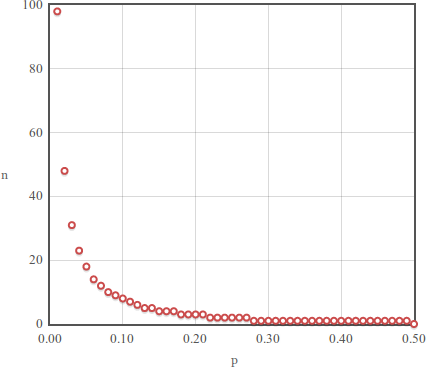
\includegraphics[width=0.6\textwidth]{../images/restriction-least-n.png}
  \caption{Least possible $n$, given a fixed $p$}
  \label{fig:sn-restriction-least-n}
\end{figure}

The second scenario, primarily of academic interest, is when $n$ is fixed and
we wish to solve for $p$. In this case, we return to
\eqref{eq:solving-the-restriction} for further factoring:

\begin{align}
  np(1-p) &\geq (1-2p)^2 \nonumber \\
  np - np^2 &\geq 1 - 4p + 4p^2 \nonumber \\
  1 - 4p + 4p^2 - np + np^2 &\leq 0 \nonumber \\
  (n+4)p^2 - (n+4)p + 1 &\leq 0 \label{eq: solving for p}.
\end{align}

We then apply the quadratic formula with $a = n+4$, $b = -(n+4)$, and $c = 1$:

\begin{align*}
  p &= \frac{(n+4) \pm \sqrt{(n+4)^2 - 4 \cdot (n+4) \cdot 1}}{2(n+4)} \\
  &= \frac{(n+4) \pm \sqrt{n^2 + 8n + 16 - 4n - 16}}{2(n+4)} \\
  &= \frac{(n+4) \pm \sqrt{n^2 + 4n}}{2(n+4)} \\
  &= \frac{n+4}{2(n+4)} \pm \frac12 \sqrt{\frac{n(n+4)}{(n+4)^2}} \\
  &= \frac12 \pm \frac12 \sqrt{\frac{n}{n+4}} \;.
\end{align*}

Let $r_1 = \frac12 - \frac12 \sqrt{\frac{n}{n+4}}$ and $r_2 = \frac12 + \frac12
\sqrt{\frac{n}{n+4}}$. (Note that $r_1 < r_2$.) Now we can rewrite \eqref{eq:
solving for p} as

\begin{equation*}
  (p - r_1)(p - r_2) \leq 0.
\end{equation*}

Examining the left hand side, when $p < r_1$, both terms are negative and so
their product is positive; when $p > r_2$, both terms are positive, again
leading the product to be positive. Therefore, our solution lies where $r_1
\leq p \leq r_2$, or more explicitly,

\begin{equation}
 \frac12 - \frac12 \sqrt{\frac{n}{n+4}} \; \leq \; p \; \leq \; \frac12 + \frac12 \sqrt{\frac{n}{n+4}} \;.
\end{equation}

Shown in figure \ref{fig:sn-restriction-p-range} as a function of $n$, this
interval grows quickly as $n$ increases, and for sufficiently large $n$, it
becomes almost $(0, 1)$. For example, when $n=100$, our interval is $(0.00971,
0.99029)$; when $n=500$, it is (0.00199, 0.99801).

\begin{figure}
  \centering
  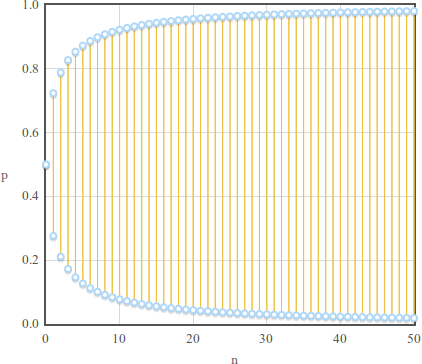
\includegraphics[width=0.6\textwidth]{../images/restriction-p-range.png}
  \caption{Range of possible $p$, given a fixed $n$}
  \label{fig:sn-restriction-p-range}
\end{figure}

Although the presence of these restrictions are somewhat disappointing, we can
console ourselves with the observation that at the same $n$ and $p$, the
skew-normal yields substantially more accurate approximations than the normal
(see section \ref{subsec:mabs}). Thus while imperfect, it is nevertheless an
improvement.

\section{Demonstrating Improved Accuracy}
\label{sec:accuracy}

Now comes the time to justify our efforts by comparing the accuracy of our
skew-normal approximation to that of the normal. Naturally, we are primarily
interested in cases where the normal approximation performs poorly, that is
binomials where $n$ is small and $p$ is either close to 0 or 1.\footnotemark

\footnotetext{Again, we examine only $p \in (0, 0.5)$. (See footnote
\ref{fnote:half-p-range}.)}

\subsection{Visual Comparison}

The first and most obvious way of judging accuracy is by visual inspection.
Figures \ref{fig:comparison-n25}, \ref{fig:comparison-n50}, and
\ref{fig:comparison-n100} compare the binomial, normal, and skew-normal at
small values of $p$ for $n=25$, $n=50$, and $n=100$, respectively.

At very small $n$ and $p$, our skew-normal curve follows the shape of the
binomial much more closely than the normal. However, as $n$ grows, the Central
Limit Theorem begins to exert its effect; even at a moderate $n = 100$ and a
smallish $p = 0.2$, the normal and skew-normal become nearly identical. Thus,
as we would expect, the skew-normal method is most valuable at small $n$ and
extreme $p$.

\subsection{Maximal Absolute Error}
\label{subsec:mabs}

Another more quantitative method of judging accuracy is comparing the maximal
absolute errors of our two approximations, defined by \citet{mabs} as

\begin{equation}
  \textnormal{MABS}(n, p) \eq \max_{k \in \{0, 1,...,n\}} \left| F_{B(n,p)} (k) -  F_{\textnormal{appr}(n,p)}(k + 0.5) \right|
\end{equation}

where $F_{B(n,p)}$ is the cdf of the binomial and $F_{\textnormal{appr}(n,p)}$
is the cdf of either the normal or skew-normal approximation; the 0.5 is a
continuity correction.

Figures \ref{fig:mabs-fixed-n} and \ref{fig:mabs-fixed-p} shows the MABS of the
skew-normal and normal approximations as a function of $p$ and $n$,
respectively. Again, the skew-normal outperforms the normal considerably in the
extreme ranges, with the two approximations converging as $n \rightarrow
\infty$ or $p \rightarrow 0.5$.

\section{Practical Resources}
\label{sec:resources}

We conclude our dicussion by offering the reader a few practical resources:

Table \ref{tab:sn-approx-table} shows estimations of $SN(\mu, \sigma, \lambda)$
for common binomial distributions.

For those with an unusual combination of $n$ and $p$ not in the table, Appendix
\ref{app:calc-sn-approx} demonstrates how to calculate the skew-normal
parameters by hand.

Finally, for rapidly approximating many binomial distributions, the author's
Python library, which was used to compute all values presented in this paper,
is freely available online:

\url{http://github.com/joycetipping/skew-normal-capstone/}

\begin{figure}
  \centering
  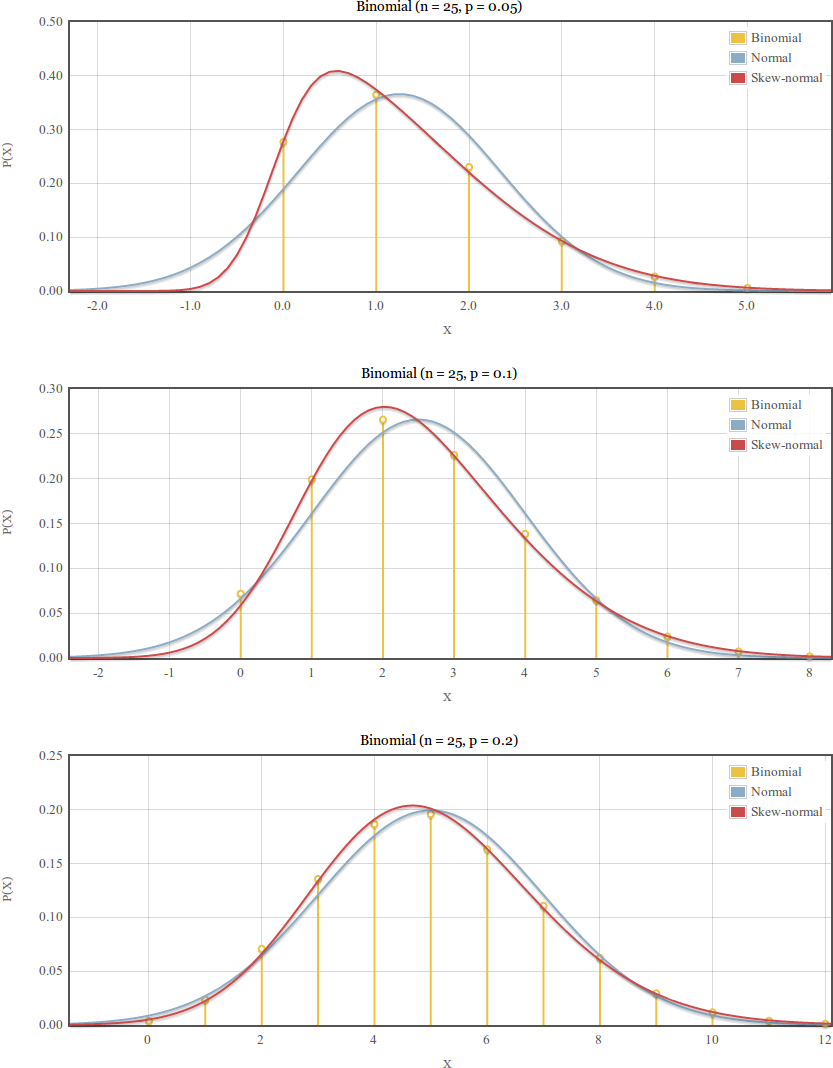
\includegraphics[width=\textwidth]{../images/comparison-n25.png}
  \caption{Binomial, normal, and skew-normal, $n=25$}
  \label{fig:comparison-n25}
\end{figure}

\begin{figure}
  \centering
  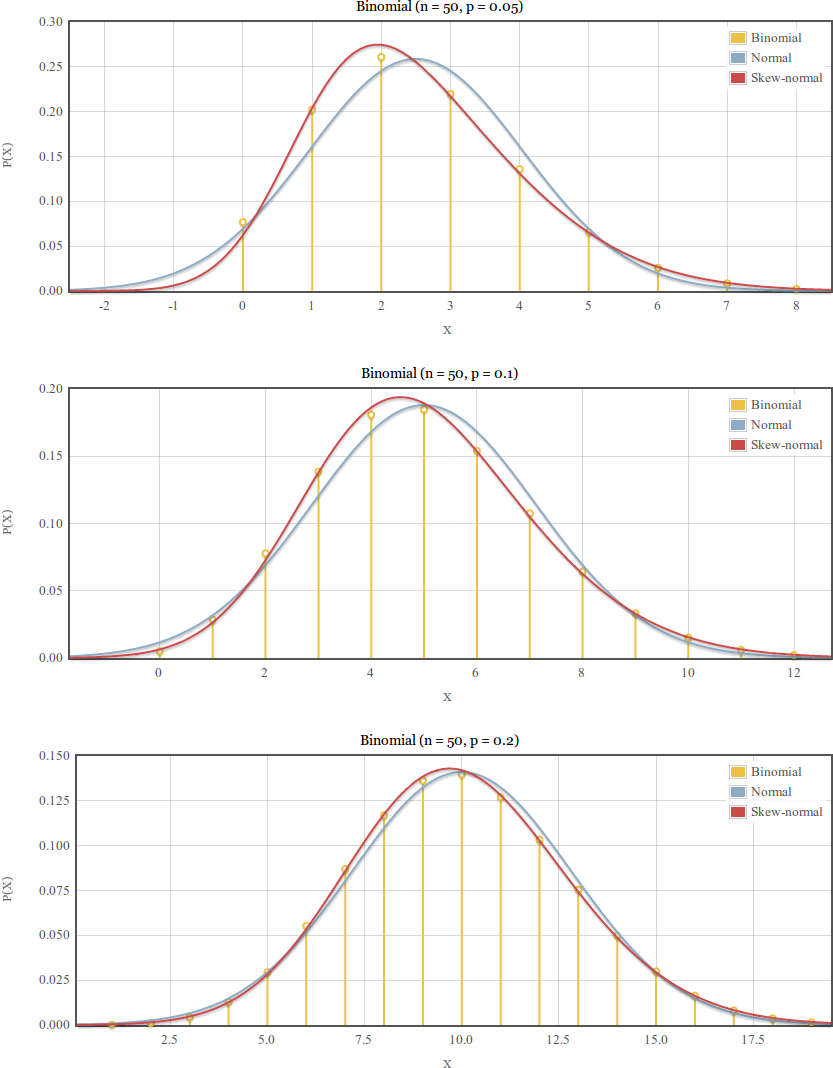
\includegraphics[width=\textwidth]{../images/comparison-n50.png}
  \caption{Binomial, normal, and skew-normal, $n=50$}
  \label{fig:comparison-n50}
\end{figure}

\begin{figure}
  \centering
  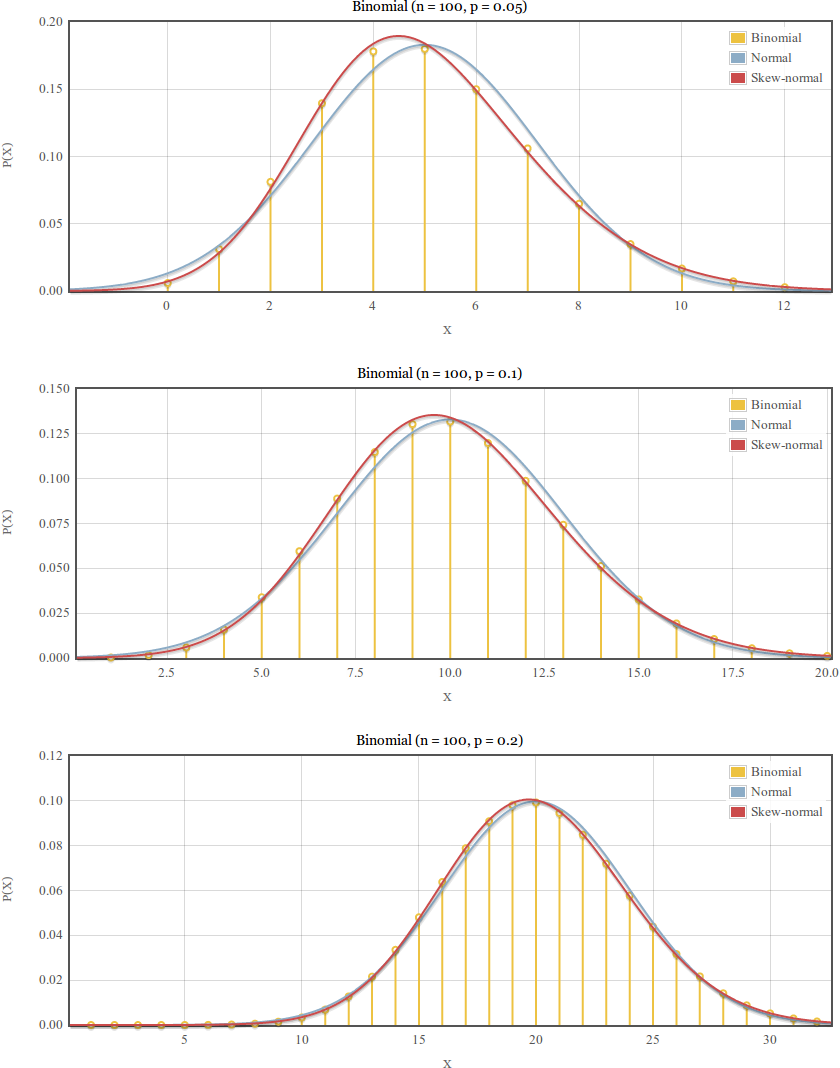
\includegraphics[width=\textwidth]{../images/comparison-n100.png}
  \caption{Binomial, normal, and skew-normal, $n=100$}
  \label{fig:comparison-n100}
\end{figure}


\begin{figure}
  \centering
  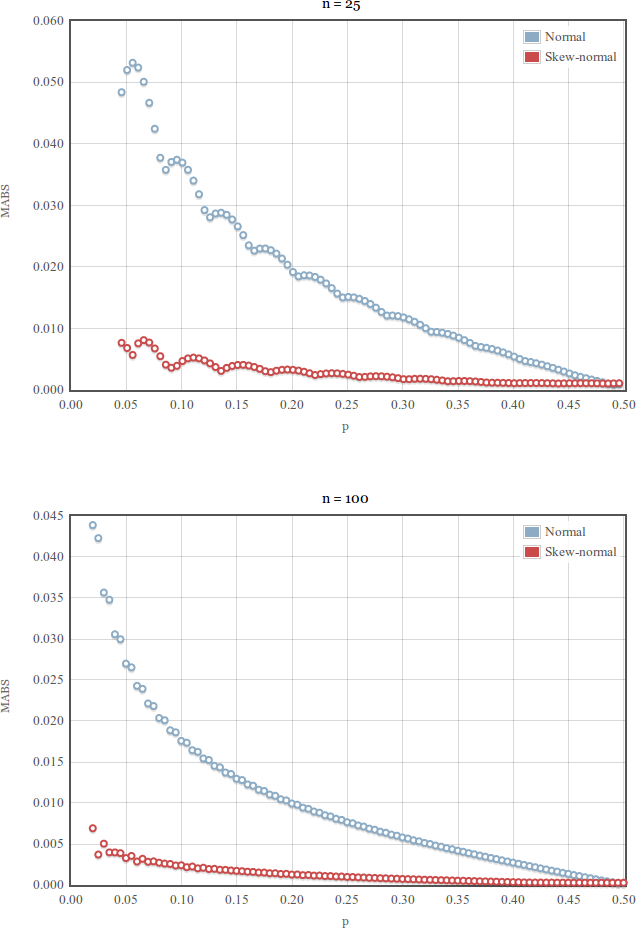
\includegraphics[width=\textwidth]{../images/mabs-fixed-n.png}
  \caption{MABS as a function of p}
  \label{fig:mabs-fixed-n}
\end{figure}

\begin{figure}
  \centering
  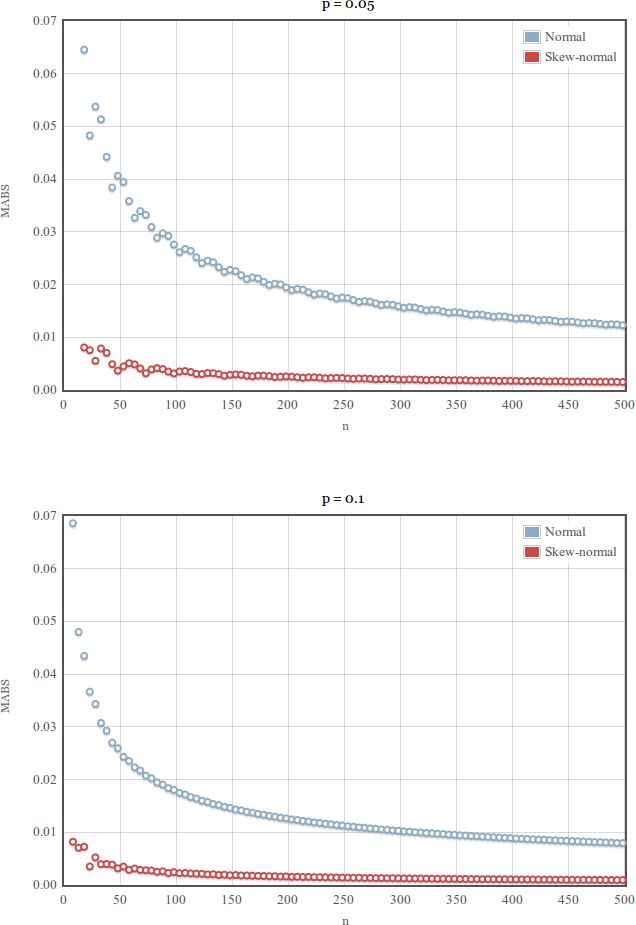
\includegraphics[width=\textwidth]{../images/mabs-fixed-p.png}
  \caption{MABS as a function of n}
  \label{fig:mabs-fixed-p}
\end{figure}

\begin{sidewaystable}
  \caption{Estimations of $SN(\mu, \sigma, \lambda)$ for $Bin(n,p)$}
  \centering
  \renewcommand{\arraystretch}{1.3}
  \begin{tabular}
    { r r | r@{}r@{,\;}r@{,\;}r@{}l r@{}r@{,\;}r@{,\;}r@{}l r@{}r@{,\;}r@{,\;}r@{}l r@{}r@{,\;}r@{,\;}r@{}l r@{}r@{,\;}r@{,\;}r@{}l }
    \hline \hline
    & & \multicolumn{5}{c}{} & \multicolumn{5}{c}{} & \multicolumn{5}{c}{$n$} & \multicolumn{5}{c}{} & \multicolumn{5}{c}{}\\
    \multirow{20}{*}{$p$} & & \multicolumn{5}{c}{25} & \multicolumn{5}{c}{50} & \multicolumn{5}{c}{100} & \multicolumn{5}{c}{250} & \multicolumn{5}{c}{500} \\
    \hline
    & 0.05 & ( & -0.11 & 1.74 & 4.56 & ) & ( & 0.79 & 2.30 & 2.54 & ) & ( & 2.85 & 3.06 & 1.86 & ) & ( & 9.58 & 4.52 & 1.38 & ) & ( & 21.32 & 6.11 & 1.15 & ) \\
    & 0.10 & ( & 0.89 & 2.20 & 2.31 & ) & ( & 2.97 & 2.94 & 1.74 & ) & ( & 7.44 & 3.94 & 1.40 & ) & ( & 21.53 & 5.88 & 1.10 & ) & ( & 45.62 & 8.01 & 0.94 & ) \\
    & 0.15 & ( & 2.02 & 2.49 & 1.79 & ) & ( & 5.32 & 3.34 & 1.43 & ) & ( & 12.25 & 4.51 & 1.19 & ) & ( & 33.77 & 6.77 & 0.96 & ) & ( & 70.30 & 9.27 & 0.82 & ) \\
    & 0.20 & ( & 3.23 & 2.67 & 1.50 & ) & ( & 7.76 & 3.61 & 1.24 & ) & ( & 17.18 & 4.89 & 1.04 & ) & ( & 46.18 & 7.39 & 0.85 & ) & ( & 95.18 & 10.16 & 0.74 & ) \\
    & 0.25 & ( & 4.49 & 2.79 & 1.29 & ) & ( & 10.28 & 3.78 & 1.09 & ) & ( & 22.20 & 5.15 & 0.93 & ) & ( & 58.71 & 7.83 & 0.76 & ) & ( & 120.22 & 10.80 & 0.67 & ) \\
    & 0.30 & ( & 5.80 & 2.85 & 1.12 & ) & ( & 12.86 & 3.88 & 0.95 & ) & ( & 27.31 & 5.32 & 0.82 & ) & ( & 71.34 & 8.12 & 0.68 & ) & ( & 145.39 & 11.24 & 0.60 & ) \\
    & 0.35 & ( & 7.17 & 2.86 & 0.96 & ) & ( & 15.50 & 3.92 & 0.83 & ) & ( & 32.49 & 5.39 & 0.72 & ) & ( & 84.09 & 8.28 & 0.60 & ) & ( & 170.70 & 11.50 & 0.53 & ) \\
    & 0.40 & ( & 8.59 & 2.83 & 0.80 & ) & ( & 18.23 & 3.89 & 0.70 & ) & ( & 37.76 & 5.39 & 0.61 & ) & ( & 96.96 & 8.32 & 0.51 & ) & ( & 196.18 & 11.60 & 0.45 & ) \\
    & 0.45 & ( & 10.12 & 2.73 & 0.61 & ) & ( & 21.08 & 3.79 & 0.53 & ) & ( & 43.21 & 5.29 & 0.47 & ) & ( & 110.07 & 8.23 & 0.40 & ) & ( & 221.93 & 11.54 & 0.35 & ) \\
    & 0.50 & ( & 12.50 & 2.50 & 0.00 & ) & ( & 25.00 & 3.54 & 0.00 & ) & ( & 50.00 & 5.00 & 0.00 & ) & ( & 125.00 & 7.91 & 0.00 & ) & ( & 250.00 & 11.18 & 0.00 & ) \\
    & 0.55 & ( & 14.88 & 2.73 & -0.61 & ) & ( & 28.92 & 3.79 & -0.53 & ) & ( & 56.79 & 5.29 & -0.47 & ) & ( & 139.93 & 8.23 & -0.40 & ) & ( & 278.07 & 11.54 & -0.35 & ) \\
    & 0.60 & ( & 16.41 & 2.83 & -0.80 & ) & ( & 31.77 & 3.89 & -0.70 & ) & ( & 62.24 & 5.39 & -0.61 & ) & ( & 153.04 & 8.32 & -0.51 & ) & ( & 303.82 & 11.60 & -0.45 & ) \\
    & 0.65 & ( & 17.83 & 2.86 & -0.96 & ) & ( & 34.50 & 3.92 & -0.83 & ) & ( & 67.51 & 5.39 & -0.72 & ) & ( & 165.91 & 8.28 & -0.60 & ) & ( & 329.30 & 11.50 & -0.53 & ) \\
    & 0.70 & ( & 19.20 & 2.85 & -1.12 & ) & ( & 37.14 & 3.88 & -0.95 & ) & ( & 72.69 & 5.32 & -0.82 & ) & ( & 178.66 & 8.12 & -0.68 & ) & ( & 354.61 & 11.24 & -0.60 & ) \\
    & 0.75 & ( & 20.51 & 2.79 & -1.29 & ) & ( & 39.72 & 3.78 & -1.09 & ) & ( & 77.80 & 5.15 & -0.93 & ) & ( & 191.29 & 7.83 & -0.76 & ) & ( & 379.78 & 10.80 & -0.67 & ) \\
    & 0.80 & ( & 21.77 & 2.67 & -1.50 & ) & ( & 42.24 & 3.61 & -1.24 & ) & ( & 82.82 & 4.89 & -1.04 & ) & ( & 203.82 & 7.39 & -0.85 & ) & ( & 404.82 & 10.16 & -0.74 & ) \\
    & 0.85 & ( & 22.98 & 2.49 & -1.79 & ) & ( & 44.68 & 3.34 & -1.43 & ) & ( & 87.75 & 4.51 & -1.19 & ) & ( & 216.23 & 6.77 & -0.96 & ) & ( & 429.70 & 9.27 & -0.82 & ) \\
    & 0.90 & ( & 24.11 & 2.20 & -2.31 & ) & ( & 47.03 & 2.94 & -1.74 & ) & ( & 92.56 & 3.94 & -1.40 & ) & ( & 228.47 & 5.88 & -1.10 & ) & ( & 454.38 & 8.01 & -0.94 & ) \\
    & 0.95 & ( & 25.11 & 1.74 & -4.56 & ) & ( & 49.21 & 2.30 & -2.54 & ) & ( & 97.15 & 3.06 & -1.86 & ) & ( & 240.42 & 4.52 & -1.38 & ) & ( & 478.68 & 6.11 & -1.15 & ) \\
  \end{tabular}
  \label{tab:sn-approx-table}
\end{sidewaystable}

\clearpage

\appendix
\section{Calculating a Skew-Normal Approximation}
\label{app:calc-sn-approx}

Although easier with a computer program, calculating estimates for $\mu$,
$\sigma$, and $\lambda$ by hand is perfectly possible. Here, we will
demonstrate using $n=25$, $p=0.1$.

By far the largest battle is finding $\lambda$. We will use Equation
\eqref{eq:solving-for-lambda} but with the simplified left hand side given by
\eqref{eq:lhs-solving-for-lambda}:

\begin{equation}
  \label{eq:calculating-lambda}
  \left( \frac{1+\lambda^2}{\lambda^2} - \frac{2}{\pi} \right)^3 \left( \frac{\pi^3}{2(4-\pi)^2} \right) = \frac{np(1-p)}{(1-2p)^2} \;.
\end{equation}

The closed-formed solution to this equation is long, hideous, and hard to work
with, so for this demonstration, we will take a numerical approach.

The left hand side of \eqref{eq:calculating-lambda} is a function of lambda;
let us denote it $f(\lambda)$. The right hand side is a constant in $n$ and
$p$; let us call it $k_{n,p}$. Our goal is to find a value of $\lambda$ such
that $f(\lambda)$ is within a certain margin of error, $e$, of $k_{n,p}$. Since
we are computing by hand, we will take $e$ to be a modest 0.01.

Recall that the sign of $\lambda$ is determined independently of the value. In
fact, $f$ is never affected by the sign of $\lambda$, as all terms are squared.
Thus, we can restrict our search for $\lambda$ to the interval $(0, \infty)$.

Next, by taking $f$'s derivative, we can show that it is monotonically
decreasing for positive $\lambda$:

\begin{align*}
  \frac{d}{d\lambda} \left[ \left( \frac{1+\lambda^2}{\lambda^2} - \frac{2}{\pi} \right)^3 \left( \frac{\pi^3}{2(4-\pi)^2} \right) \right] &= \left( \frac{\pi^3}{2(4-\pi)^2} \right) \cdot
    3 \left( \frac{1+\lambda^2}{\lambda^2} - \frac{2}{\pi} \right)^2 \cdot \left( \frac{2\lambda}{\lambda^2} - \frac{2(1+\lambda^2)}{\lambda^3} \right) \\
  &= \left( \frac{\pi^3}{2(4-\pi)^2} \right) \cdot 3 \left( \frac{1+\lambda^2}{\lambda^2} - \frac{2}{\pi} \right)^2 \cdot
    \left( \cancel{\frac{2}{\lambda}} - \frac{2}{\lambda^3} - \cancel{\frac{2}{\lambda}} \right) \\
  &= \underbrace{\left( \frac{\pi^3}{2(4-\pi)^2} \right) \cdot 3 \left( \frac{1+\lambda^2}{\lambda^2} - \frac{2}{\pi} \right)^2}_\textnormal{Always positive} \quad \cdot \quad
     \underbrace{\left( -\frac{2}{\lambda^3} \right)}_{\mathclap{\textnormal{Negative when $\lambda > 0$}}}.
\end{align*}

This convenient fact allows us to find lower and upper bounds for $\lambda$ and
repeatedly bisect our interval until we are within $e$ of $k_{n,p}$.

(For the following calculations, it is helpful to keep in mind that because $f$
is decreasing in $\lambda$, smaller values of $\lambda$ will produce larger
values of $f$, and vice versa.)
    
\begin{enumerate}
  \item \textit{Find $k_{n,p}$.}
  
    Our value: $\displaystyle k_{n,p} = \frac{25 \cdot 0.1 \cdot 0.9}{(1 - 2\cdot0.1)^2} = 3.5156$.

  \item \textit{Find $a$ and $b$ such that $f(a) > k_{n,p} > f(b)$.}
    
    Our values: $a=1$, $b=3$.
  
  \item \textit{Repeatedly bisect $(a,b)$ until $f(c)$ is within $e$ of $k_{n,p}$.}

    Calculate $c=\frac{a+b}{2}$.

    \begin{itemize}
      \item If $f(c) \leq k_{n,p} - 0.01$, we need a small value of $c$, so we
      take our new interval to be $(a, c)$.
    
      \item If $f(c) \geq k_{n,p} + 0.01$, we need a larger value of $c$, so we
      take our new interval to be $(c, b)$.
    \end{itemize}
    
    Repeat this step until $f(c)$ is within $e$ of $k_{n,p}$, or more precisely
    $k_{n,p} - 0.01 < f(c) < k_{n,p} + 0.01$.

    The following table shows our iterations:

    \renewcommand{\arraystretch}{1.3}
    \begin{center}
      \begin{tabular}{c c c c c c c}
        Iteration & $a$  & $b$   & $c$    & $f(c)$ & $f(c) \leq k_{n,p} - 0.01$ & $f(c) \geq k_{n,p} + 0.01$ \\
        \hline
        1         & 2.00 & 3.000 & 2.5000 & 3.0164 & True                       & False \\
        2         & 2.00 & 2.500 & 2.2500 & 3.7129 & False                      & True \\
        3         & 2.25 & 2.500 & 2.3750 & 3.3252 & True                       & False \\
        4         & 2.25 & 2.375 & 2.3125 & 3.5076 & False                      & False \\
      \end{tabular}
    \end{center}

    We take the last value of $c$: 2.3125.

  \item \textit{Find the sign of $(1-2p)$.}

    Our $p = 0.1 \Ra (1 - 2\cdot0.1) = 0.8 \Ra$ positive.

  \item \textit{Final answer: \{sign of $(1-2p)$\}$\lambda$}

    Our final answer: $\lambda = 2.3125$.
\end{enumerate}

Once we have $\lambda$, we can easily find $\sigma$:

\begin{equation*}
  \sigma = \sqrt{\frac{np(1-p)}{1 - \frac{2}{\pi} \cdot \frac{\lambda^2}{1 + \lambda^2}}} = \sqrt{\frac{25 \cdot 0.1 \cdot 0.9}{1 - \frac{2}{\pi} \cdot \frac{2.3125^2}{1 + 2.3125^2}}} = 2.2029. \\
\end{equation*}

And with $\lambda$ and $\sigma$, we can also find $\mu$:

\begin{equation*}
  \mu = np - \sigma \cdot \sqrt{\frac{2}{\pi}} \cdot \frac{\lambda}{\sqrt{1 + \lambda^2}} = 25 \cdot 0.1 - 2.2029 \cdot \sqrt{\frac{2}{\pi}} \cdot \frac{2.3125}{\sqrt{1 + 2.3125^2}} = 0.8867.
\end{equation*}

\clearpage
\bibliography{bibliography.bib}
\bibliographystyle{plainnat}
\end{document}
